% !TeX program = xelatex
% !TeX encoding = UTF-8
% !TeX TXS-program:compile = txs:///xelatex | txs:///xelatex
\documentclass[aspectratio=169, table, 12pt]{beamer}
% Preamble bersama seluruh slide mata kuliah ini.
% Dipanggil dari slides/sessionXX/sessionXX.tex tepat sesudah baris
% \documentclass[aspectratio=169, table, 12pt]{beamer}
% Paket tambahan yang hanya dibutuhkan satu sesi ditulis di berkas sesi itu.

\usepackage{colortbl}
\usepackage{xcolor}
\usepackage{listings}
\usepackage{tabularx}
\usepackage{booktabs}
\usepackage{tikz}
\usepackage{pgfplots}
\pgfplotsset{compat=1.18}
\usetikzlibrary{arrows.meta, positioning, calc, fit, shapes.geometric,
	shapes.multipart, backgrounds, matrix, chains, trees}

\makeatletter
\def\input@path{{../theme/}}
\makeatother
\graphicspath{{../theme/}{../../figures/}}
\usetheme{Pradita}

\definecolor{praditagreen}{RGB}{37, 113, 71}

% Tema membuat garis tabel berwarna putih. Dikembalikan agar tabel terbaca.
\arrayrulecolor{black}
\setlength{\arrayrulewidth}{0.5pt}

\lstdefinelanguage{yaml}{
	basicstyle=\ttfamily\scriptsize,
	keywordstyle=\color{blue}\bfseries,
	commentstyle=\color{gray}\itshape,
	stringstyle=\color{red},
	showstringspaces=false,
	breaklines=true,
	frame=lines,
	numbers=none,
	backgroundcolor=\color{lightgray!10},
	tabsize=2,
	morecomment=[l]{\#}
}

\lstdefinelanguage{json}{
	basicstyle=\ttfamily\scriptsize,
	stringstyle=\color{red},
	commentstyle=\color{gray},
	breaklines=true,
	showstringspaces=false,
	tabsize=2,
	numbers=none,
	frame=lines,
	backgroundcolor=\color{lightgray!10},
	string=[s]{"}{"}
}

\lstdefinelanguage{bash}{
	keywords={},
	basicstyle=\ttfamily\scriptsize,
	ndkeywords={docker, kubectl, helm, curl, git, terraform},
	ndkeywordstyle=\color{purple}\bfseries,
	sensitive=true,
	commentstyle=\color{gray},
	numbers=none,
	breaklines=true,
	frame=lines,
	backgroundcolor=\color{lightgray!10},
	tabsize=2,
	comment=[l]{\#},
	showstringspaces=false
}

\lstdefinelanguage{http}{
	keywords={GET, POST, PUT, PATCH, DELETE, HEAD, OPTIONS, HTTP},
	basicstyle=\ttfamily\scriptsize,
	keywordstyle=\color{blue}\bfseries,
	sensitive=true,
	numbers=none,
	breaklines=true,
	frame=lines,
	backgroundcolor=\color{lightgray!10},
	tabsize=2,
	showstringspaces=false
}

\subtitle{IT40613 · Digital Platform \& API Economy}
\author{\textbf{Alfa Yohannis}}


% Tanda kutip tunggal dibaca sebagai teks, supaya tanda pagar pada $ref tidak dianggap komentar.
\lstdefinestyle{ch09yaml}{language=yaml, morestring=[b]', basicstyle=\ttfamily\scriptsize}

\title{\Huge Desain Kontrak API\\ \vspace{10pt} dengan OpenAPI}
\date{Pertemuan 09}

\begin{document}
\frame{\titlepage}

\begin{frame}
  \frametitle{Isi Pertemuan}
  \vspace{14pt}
  \begin{columns}[t]
    \column{0.5\textwidth}
    {\small\tableofcontents[sections={1-4}]}

    \column{0.5\textwidth}
    {\small\tableofcontents[sections={5-9}]}
  \end{columns}
\end{frame}

\begin{frame}{\hfill}
  \centering
  \Huge{\textbf{Vendor berkata berhasil.\\Klinik masih menelepon.\\Di mana arti berhasil\\ditulis?}}
\end{frame}

\section{Tujuan dan Konteks}

\begin{frame}{{\Large Tujuan Pembelajaran}}
  \vspace{10pt}
  \begin{itemize}
    \item Menjelaskan pendekatan \textit{contract-first} dan manfaatnya bagi kerja sama dengan vendor dan mitra.
    \item Membaca dan meninjau kontrak OpenAPI dari sisi bisnis maupun teknis.
    \item Menyusun kontrak OpenAPI sederhana untuk satu API prioritas.
  \end{itemize}
\end{frame}

\begin{frame}{{\Large Diagram Konsep Bab 9}}
  \centering
  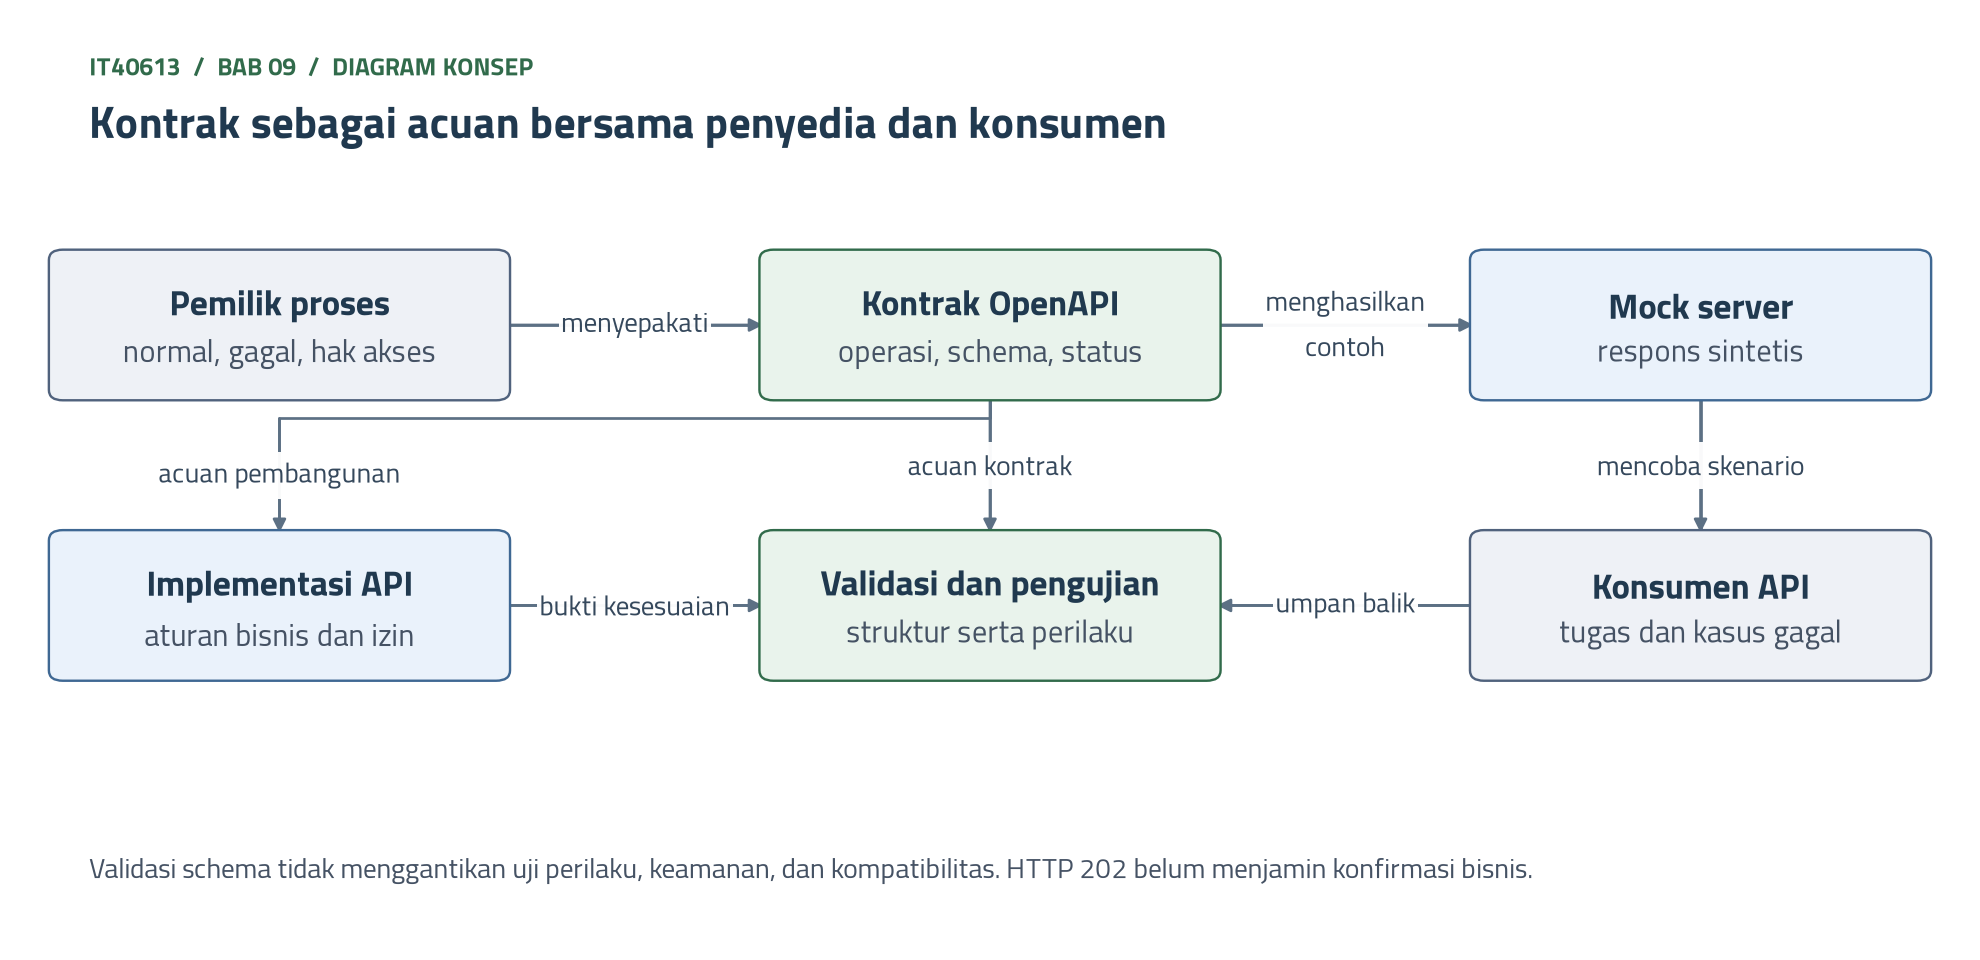
\includegraphics[width=0.96\textwidth,height=0.77\textheight,keepaspectratio]{../../figures/ch09-diagram-konsep.png}
\end{frame}

\begin{frame}{{\Large Masukan dari Bab Sebelumnya}}
  \footnotesize
  \begin{tabularx}{\textwidth}{>{\raggedright\arraybackslash}p{1.3cm} >{\raggedright\arraybackslash}X >{\raggedright\arraybackslash}p{5.0cm}}
    \hline
    \textbf{Asal} & \textbf{Temuan yang dipakai} & \textbf{Kegunaan di sini} \\ \hline
    Bab 1, 5 & \texttt{/jadwal-dokter}, \texttt{/janji-temu}, kode 201, 202, 409, 429 & Bahan operasi dan jawaban \\ \hline
    Bab 4 & INT-03: 28.000 janji per bulan, 140 tabel. 4 jam per perubahan per klinik & Masalah dan biaya perubahan \\ \hline
    Bab 6 & \textit{Scope} seperti \texttt{hasil.baca}, hak atas objek & Bagian \texttt{security} \\ \hline
    Bab 7, 8 & Kunjungan, janji temu, dan Encounter tertukar & Kosakata kontrak \\ \hline
    Bab 8 & API-01, 40 klinik, 180 panggilan dari kuota 300 & API prioritas \\ \hline
  \end{tabularx}

  \vspace{8pt}
  \small Tarif Rp60.000 per jam, Rp45 juta per antarmuka, 20 sambungan aktif Rp900 juta per tahun.
\end{frame}

\section{Kontrak dan Contract-First}

\begin{frame}{{\Large Kontrak API sebagai Perjanjian}}
  \vspace{8pt}
  \begin{itemize}
    \item Kesepakatan tertulis antara penyedia dan konsumen tentang perilaku antarmuka.
    \item Memuat operasi, data, autentikasi, respons, dan kondisi gagal.
    \item \textit{Contract-first}: disepakati sebelum implementasi rinci.
    \item Kontrak teknis dibaca bersama aturan bisnis, misalnya kapan slot terkunci.
    \item Zimmermann dkk.: pola API Description, juga disebut Explicit Service Contract.
  \end{itemize}
  \vspace{6pt}
  {\small Analogi: gambar kerja rumah disepakati pembeli dan pelaksana sebelum tembok berdiri.}
\end{frame}

\begin{frame}{{\Large Dua Contoh Berangka}}
  \vspace{8pt}
  \begin{itemize}
    \item 202 hanya berarti diterima untuk diproses. RFC 9110: permintaan masih mungkin tidak dijalankan.
    \item Misalkan 202 ditampilkan sebagai berhasil dan 2 persen berakhir slot penuh: 48 pasien per hari tanpa janji, 200 jam per bulan, Rp144 juta per tahun.
    \item Misalkan salah arti ditemukan saat tinjauan: 5 orang, 2 jam, Rp600.000.
    \item Ditemukan sesudah dibangun: 80 jam vendor dan 160 jam klinik, Rp14,4 juta.
    \item Temuan yang sama menjadi 24 kali lebih mahal.
  \end{itemize}
\end{frame}

\begin{frame}{{\Large Contract-First pada Garis Waktu}}
  \centering
  \eadiagram{../../figures/ch09-alur-contract-first.tex}
\end{frame}

\begin{frame}{{\Large Membaca Kontrak Tanpa Memprogram}}
  \footnotesize
  \begin{tabularx}{\textwidth}{>{\raggedright\arraybackslash}X >{\raggedright\arraybackslash}p{2.6cm} >{\raggedright\arraybackslash}X}
    \hline
    \textbf{Pertanyaan pembaca} & \textbf{Bagian kontrak} & \textbf{Jawaban pada API-01} \\ \hline
    Siapa penanggung jawabnya? & \texttt{info} & Manajer Layanan Rawat Jalan \\ \hline
    Apa yang boleh dilakukan? & \texttt{paths} & Cari jadwal, buat janji, baca status, batalkan \\ \hline
    Data apa yang masuk dan keluar? & \textit{schema} & Slot dan nomor pasien, tanpa rekam medis \\ \hline
    Apa arti berhasil? & \texttt{responses} 2xx & 201 terkonfirmasi, 202 menunggu \\ \hline
    Apa arti gagal? & \texttt{responses} 4xx, 5xx & 409 slot terisi, tawarkan slot lain \\ \hline
    Siapa yang boleh memanggil? & \texttt{security} & \textit{Scope} \texttt{janji.tulis} \\ \hline
  \end{tabularx}
\end{frame}

\begin{frame}{{\Large Yang Sering Tertukar dan Tradeoff}}
  \footnotesize
  \begin{tabularx}{\textwidth}{>{\raggedright\arraybackslash}p{2.4cm} >{\raggedright\arraybackslash}X >{\raggedright\arraybackslash}X}
    \hline
    \textbf{Unsur} & \textbf{\textit{Contract-first}} & \textbf{\textit{Code-first}} \\ \hline
    Kesepakatan & Sebelum pembangunan & Sesudah kode berjalan \\ \hline
    Risiko utama & Waktu rapat, kontrak dapat basi & Salah arti ditemukan terlambat \\ \hline
    Cocok untuk & Banyak konsumen, vendor terpisah & API internal satu tim \\ \hline
  \end{tabularx}

  \vspace{8pt}
  \small
  \begin{itemize}
    \item Kontrak API mengatur perilaku. Perjanjian kerja sama mengatur harga dan tanggung jawab hukum.
    \item Misalkan tiga sesi 2 jam dengan 5 orang: 30 jam, Rp1,8 juta.
    \item Postman: 82 persen mengadopsi \textit{API-first} pada tingkat tertentu, 25 persen sepenuhnya. Pengakuan responden, dan Postman menjual alat API.
  \end{itemize}
\end{frame}

\begin{frame}{{\Large Kasus Medikara: Arti Berhasil pada API-01}}
  \vspace{8pt}
  \begin{itemize}
    \item 201: slot terkunci di SIMRS. Layar menulis ``janji terkonfirmasi''.
    \item 202: masih diproses. Layar menulis ``menunggu kepastian''.
    \item 409: slot terisi, janji tidak dibuat. Aplikasi menawarkan slot lain.
    \item Misalkan 5 persen berakhir di 202: 120 janji, 600 panggilan baca status per hari, 195 panggilan per klinik dari kuota 300.
    \item Target telepon 10 ke 2 persen: 300 menjadi 60 jam per bulan, hemat Rp172,8 juta per tahun bila tercapai.
  \end{itemize}
\end{frame}

\section{Sumber Daya dan Pola}

\begin{frame}{{\Large Pemodelan Sumber Daya}}
  \vspace{8pt}
  \begin{itemize}
    \item Sumber daya adalah hal yang dikenali pengguna, bukan tabel.
    \item \texttt{GET /jadwal-dokter} mengembalikan slot. \texttt{POST /janji-temu} tetap memeriksa slot.
    \item Daftar slot dapat berumur 5 menit: 280 bentrok per bulan dijawab 409.
    \item Pengenal \texttt{JT-40771} stabil, tetapi bukan bukti kewenangan.
    \item Hanya memeriksa token: 300 per hari, 9.000 nomor dalam 30 hari dapat dicoba.
  \end{itemize}
  \vspace{6pt}
  {\small Analogi: nomor antrean tetap dikenali walaupun petugas loket berganti.}
\end{frame}

\begin{frame}{{\Large Kosakata Kontrak API-01}}
  \footnotesize
  \begin{tabularx}{\textwidth}{>{\raggedright\arraybackslash}p{2.4cm} >{\raggedright\arraybackslash}X >{\raggedright\arraybackslash}p{3.1cm} >{\raggedright\arraybackslash}p{2.1cm}}
    \hline
    \textbf{Kata} & \textbf{Arti dalam kontrak} & \textbf{Bukan berarti} & \textbf{Padanan FHIR} \\ \hline
    Slot & Rentang waktu yang dapat dipesan & Janji temu & Slot \\ \hline
    Janji temu & Pemesanan pasien atas satu slot & Kunjungan & Appointment \\ \hline
    Kunjungan & Pertemuan yang terjadi, di luar API-01 & Janji temu & Encounter \\ \hline
    Terkonfirmasi & Slot sudah terkunci di SIMRS & Sudah diterima & Tidak dipetakan \\ \hline
    Menunggu & Diterima, hasil belum pasti & Janji pasti ada & Tidak dipetakan \\ \hline
  \end{tabularx}

  \vspace{8pt}
  \small Kanvas Bab 8 menyebut lima kata kerja, kontrak memuat empat operasi. Memilih slot terjadi di layar konsumen, dan mengunci slot adalah bagian dari membuat janji.
\end{frame}

\begin{frame}{{\Large Status Janji Temu}}
  \centering
  \eadiagram{../../figures/ch09-status-janji-temu.tex}
\end{frame}

\begin{frame}{{\Large Pola Desain API}}
  \scriptsize
  \begin{tabularx}{\textwidth}{>{\raggedright\arraybackslash}p{3.6cm} >{\raggedright\arraybackslash}X >{\raggedright\arraybackslash}p{4.4cm}}
    \hline
    \textbf{Pola} & \textbf{Pertanyaan yang dijawab} & \textbf{Pada API-01} \\ \hline
    Retrieval Operation & Bagaimana mengambil informasi? & \texttt{GET /jadwal-dokter} \\ \hline
    State Creation Operation & Bagaimana melaporkan hal yang perlu diproses? & \texttt{POST /janji-temu} \\ \hline
    State Transition Operation & Bagaimana memicu perubahan keadaan? & \texttt{DELETE /janji-temu/\{id\}} \\ \hline
    Pagination & Bagaimana mengirim banyak data? & \texttt{batas} dan \texttt{kursor} \\ \hline
    Error Report & Bagaimana memberi tahu kesalahan? & \textit{Problem Details} \\ \hline
    Rate Limit & Bagaimana mencegah pemakaian berlebihan? & 300 per hari per klinik, kode 429 \\ \hline
  \end{tabularx}

  \vspace{8pt}
  \small Analogi: pola jahit. Misalkan Request Bundle diusulkan vendor: panggilan turun dari 60 ke 1, tetapi cadangan kuota masih 120. Masalahnya belum ada, sehingga pola ditolak.
\end{frame}

\section{Galat dan Pagination}

\begin{frame}{{\Large Problem Details (RFC 9457)}}
  \vspace{8pt}
  \begin{itemize}
    \item Objek JSON dengan jenis media \texttt{application/problem+json}.
    \item Lima bidang: \texttt{type}, \texttt{status}, \texttt{title}, \texttt{detail}, \texttt{instance}.
    \item \texttt{type} menentukan tindakan konsumen, kalimat ditujukan kepada manusia.
    \item Pesan tidak boleh membuka data sensitif atau rincian internal.
    \item Misalkan 280 bentrok per bulan berakhir telepon 6 menit: 28 jam per bulan, Rp20,16 juta per tahun.
  \end{itemize}
  \vspace{6pt}
  {\small Analogi: surat penolakan menjelaskan masalah tanpa membuka arsip internal petugas.}
\end{frame}

\begin{frame}[fragile]{{\Large Contoh Galat Slot Terisi}}
\begin{lstlisting}[style=ch09yaml]
    SlotTerisi:
      summary: Slot sudah dipakai pasien lain.
      value:
        type: https://api.medikara.example/masalah/slot-terisi
        title: Slot sudah terisi
        status: 409
        detail: Slot BKS-20261102-0915 sudah terisi. Pilih slot lain.
        instance: /kejadian/MSL-20261102-00731
\end{lstlisting}

  \vspace{6pt}
  \small Berkas: \berkas{sources/chapter09/kontrak-api-01-janji-temu.yaml}. Jawaban dikirim sebagai JSON dengan isi yang sama. Petugas cukup menyebut nomor \texttt{instance}, tanpa nama pasien.
\end{frame}

\begin{frame}{{\Large Model Galat API-01}}
  \scriptsize
  \begin{tabularx}{\textwidth}{>{\raggedright\arraybackslash}p{0.7cm} >{\raggedright\arraybackslash}p{4.3cm} >{\raggedright\arraybackslash}X >{\raggedright\arraybackslash}p{3.3cm}}
    \hline
    \textbf{Kode} & \textbf{Tipe masalah} & \textbf{Pesan bagi petugas} & \textbf{Tindakan konsumen} \\ \hline
    400 & \texttt{pasien-tidak-dapat-dipakai} & Periksa kartu pasien & Jangan menebak nomor \\ \hline
    401 & \texttt{token-tidak-sah} & Akses kedaluwarsa & Minta token baru \\ \hline
    404 & \texttt{janji-tidak-ditemukan} & Janji tidak ditemukan & Periksa nomor janji \\ \hline
    409 & \texttt{slot-terisi} & Slot sudah terisi. Pilih slot lain & Tawarkan slot lain \\ \hline
    429 & \texttt{kuota-habis} & Kuota hari ini habis & Tunda, \texttt{Retry-After} \\ \hline
    503 & \texttt{simrs-tidak-tersedia} & Bukan berarti tidak ada dokter & Coba lagi, \texttt{Retry-After} \\ \hline
  \end{tabularx}

  \vspace{8pt}
  \small Jadwal kosong 7 sampai 14 hari per tahun saat SIMRS diperbarui: 16.800 sampai 33.600 pemesanan keliru bila dijawab 200. Janji klinik lain dijawab 404, karena RFC 9110 membolehkan 404 untuk menyembunyikan keberadaan.
\end{frame}

\begin{frame}{{\Large Pagination dan Penyaringan}}
  \vspace{8pt}
  \begin{itemize}
    \item \textit{Pagination} membatasi hasil, penyaringan mempersempit kebutuhan.
    \item Misalkan 480 slot, 20 per halaman: 24 halaman, 1.440 panggilan per hari, di atas kuota 300.
    \item \texttt{spesialis=anak}: 24 slot, 2 halaman. Satu pemesanan tetap 3 panggilan, 180 per hari.
    \item Satu pemesanan tiap 1,5 menit per rumah sakit: \textit{offset} dapat melewatkan slot.
    \item \textit{Cursor} tidak bergantung pada posisi mutlak, tetapi tidak dapat melompat halaman.
  \end{itemize}
  \vspace{6pt}
  {\small Analogi: kartu katalog. Laci adalah penyaringan, lembar kartu adalah halaman.}
\end{frame}

\section{Kompatibilitas}

\begin{frame}{{\Large Kompatibilitas dan Perubahan yang Merusak}}
  \vspace{8pt}
  \begin{itemize}
    \item Dinilai dari kontrak yang dijanjikan dan perilaku klien nyata.
    \item \texttt{pasien} dari teks menjadi angka: 160 jam di klinik, Rp9,6 juta, ditambah Rp8 juta vendor, atau Rp17,6 juta.
    \item Bidang opsional \texttt{lokasi}: misalkan 5 dari 40 klinik memakai validasi ketat, 20 jam, Rp1,2 juta.
    \item Hyrum's Law: semua perilaku yang teramati akan diandalkan seseorang.
    \item Konsumen wajib mengabaikan bidang jawaban yang tidak dikenal.
  \end{itemize}
  \vspace{6pt}
  {\small Analogi: ukuran kemasan baru dapat mengganggu rak toko walaupun isinya lebih baik.}
\end{frame}

\begin{frame}{{\Large Jenis Perubahan}}
  \scriptsize
  \begin{tabularx}{\textwidth}{>{\raggedright\arraybackslash}X >{\raggedright\arraybackslash}p{1.7cm} >{\raggedright\arraybackslash}p{2.1cm} >{\raggedright\arraybackslash}X}
    \hline
    \textbf{Perubahan} & \textbf{Arah} & \textbf{Penilaian} & \textbf{Alasan} \\ \hline
    Mengganti tipe \texttt{pasien} & Keduanya & Merusak & Validasi klien gagal \\ \hline
    Menambah bidang wajib & Permintaan & Merusak & Klien lama ditolak 400 \\ \hline
    Melonggarkan batas 50 ke 100 slot & Permintaan & Umumnya aman & Permintaan lama tetap sah \\ \hline
    Menambah bidang opsional & Jawaban & Bersyarat & Uji klien ketat \\ \hline
    Menambah nilai status baru & Jawaban & Bersyarat & Daftar status klien tertutup \\ \hline
    Menambah operasi baru & Tidak ada & Aman & Klien lama tidak memanggilnya \\ \hline
    Mengubah arti 201 & Jawaban & Merusak & Alat tidak melihatnya \\ \hline
  \end{tabularx}
\end{frame}

\begin{frame}{{\Large Peta Keputusan Perubahan}}
  \centering
  \eadiagram{../../figures/ch09-peta-keputusan.tex}
\end{frame}

\begin{frame}{{\Large Membaca Bukti dengan Hati-hati}}
  \footnotesize
  \begin{tabularx}{\textwidth}{>{\raggedright\arraybackslash}p{2.8cm} >{\raggedright\arraybackslash}X >{\raggedright\arraybackslash}p{3.8cm}}
    \hline
    \textbf{Sumber} & \textbf{Temuan} & \textbf{Batas} \\ \hline
    Xavier dkk.\ 2017 & 317 pustaka, 9 ribu rilis, 260 ribu klien. 14,78 persen perubahan merusak, 2,54 persen klien terdampak & Pustaka Java, klien memilih kapan memperbarui \\ \hline
    Espinha dkk.\ 2014 & Enam pengembang, empat penyedia API web. Penyedia dapat mematikan versi & Studi eksploratif \\ \hline
    Robinson 2006 & Kontrak disusun dari harapan konsumen yang berjalan & Harapan harus dirawat \\ \hline
  \end{tabularx}

  \vspace{8pt}
  \small Prosedur: Version Identifier, Semantic Versioning, Two in Production. Masa transisi diputuskan di Bab 10.
\end{frame}

\section{Struktur OpenAPI 3.2}

\begin{frame}{{\Large Struktur OpenAPI 3.2}}
  \vspace{8pt}
  \begin{itemize}
    \item Wajib: \texttt{openapi}, \texttt{info}, dan minimal satu dari \texttt{paths}, \texttt{components}, \texttt{webhooks}.
    \item \textit{Schema} merupakan perluasan JSON Schema Draft 2020-12.
    \item API-01: 3 jalur, 4 operasi, 9 \textit{schema}, 8 jawaban galat bersama.
    \item Spesifikasi adalah dokumen kontrak, bukan mekanisme otorisasi.
    \item Satu klinik memesan 60 dari 2.400 janji. Tanpa cek objek, 2.340 janji lain terbuka.
  \end{itemize}
  \vspace{6pt}
  {\small Analogi: daftar isi dan aturan formulir tidak menggantikan pemeriksaan petugas.}
\end{frame}

\begin{frame}{{\Large Anatomi Kontrak OpenAPI}}
  \centering
  \eadiagram{../../figures/ch09-anatomi-openapi.tex}
\end{frame}

\begin{frame}[fragile]{{\Large Potongan Operasi Membuat Janji Temu}}
\begin{lstlisting}[style=ch09yaml]
      responses:
        '201':
          description: Janji terkonfirmasi. Slot sudah terkunci di SIMRS.
          headers:
            Location:
              $ref: '#/components/headers/LokasiJanji'
          content:
            application/json:
              schema:
                $ref: '#/components/schemas/JanjiTemu'
        '202':
          description: Permintaan diterima. Janji belum terkonfirmasi.
\end{lstlisting}

  \vspace{4pt}
  \small Berkas: \berkas{sources/chapter09/kontrak-api-01-janji-temu.yaml}. Kalimat \texttt{description} adalah keputusan pemilik proses. Data contoh bersifat sintetis.
\end{frame}

\begin{frame}{{\Large Batas Kontrak}}
  \footnotesize
  \begin{tabularx}{\textwidth}{>{\raggedright\arraybackslash}p{2.4cm} >{\raggedright\arraybackslash}X >{\raggedright\arraybackslash}X}
    \hline
    \textbf{Bagian} & \textbf{Yang dinyatakan} & \textbf{Yang tidak dijamin} \\ \hline
    \texttt{paths} & Operasi menurut rancangan & Sudah dibangun atau cukup cepat \\ \hline
    \textit{Schema} & Bentuk data & Kebenaran isi, misalnya slot sudah lewat \\ \hline
    \texttt{responses} & Kode dan arti yang dijanjikan & Server benar-benar menjawab demikian \\ \hline
    \texttt{security} & \textit{Scope} yang dibutuhkan & Pemeriksaan token dan hak atas objek \\ \hline
  \end{tabularx}

  \vspace{8pt}
  \small Spectral 6.17.0 dan Prism 5.14.2 sudah dicoba dan menerima kontrak 3.2.0. Bila versi alat lain menolaknya, kontrak API-01 tetap valid sebagai 3.1.1, karena tidak memakai bidang khusus 3.2.
\end{frame}

\section{AsyncAPI}

\begin{frame}{{\Large AsyncAPI untuk API Berbasis Event}}
  \vspace{8pt}
  \begin{itemize}
    \item Mendeskripsikan API berbasis pesan, tidak terikat protokol.
    \item Isi: \textit{channel}, \textit{message}, \textit{operation} (\texttt{send} atau \texttt{receive}), dan komponen.
    \item 240 hasil per hari. Pesan hanya memuat pengenal, tanpa isi hasil.
    \item 1 dari 10.000 pada 72.000 hasil per tahun: sekitar 7 hasil salah sasaran.
    \item 5 kiriman ulang per hari: 125 notifikasi ganda per bulan bila tanpa pengenal kejadian.
  \end{itemize}
  \vspace{6pt}
  {\small Analogi: alamat kotak surat dan bentuk surat berbeda dari janji kurir.}
\end{frame}

\begin{frame}{{\Large OpenAPI dan AsyncAPI}}
  \footnotesize
  \begin{tabularx}{\textwidth}{>{\raggedright\arraybackslash}p{2.8cm} >{\raggedright\arraybackslash}X >{\raggedright\arraybackslash}X}
    \hline
    \textbf{Unsur} & \textbf{OpenAPI 3.2} & \textbf{AsyncAPI 3.1} \\ \hline
    Yang memulai & Konsumen bertanya & Pengirim memberi tahu \\ \hline
    Unit kontrak & Jalur dan operasi & \textit{Channel}, \textit{message}, \textit{operation} \\ \hline
    Arti berhasil & Kode status & Perlu aturan terpisah \\ \hline
    Contoh Medikara & \texttt{POST /janji-temu} & Pesan \texttt{hasil.tersedia} \\ \hline
  \end{tabularx}

  \vspace{8pt}
  \small Apakah API-01 memerlukan pesan? Belum. Pesan menghemat 480 dari 600 panggilan, tetapi satu klinik hanya memakai 15 panggilan, dan kuotanya masih bersisa 105.
\end{frame}

\section{Tinjauan dan Mock Server}

\begin{frame}{{\Large Tinjauan Desain dan Mock Server}}
  \vspace{8pt}
  \begin{itemize}
    \item Tinjauan menguji skenario normal, salah masukan, hak kurang, dan dependensi gagal.
    \item \textit{Mock server} memberi jawaban perkiraan, bukan bukti kemampuan sistem nyata.
    \item \textit{Linter} memeriksa aturan otomatis, sedangkan makna memerlukan percakapan.
    \item Misalkan 5 klinik, 6 skenario, 20 menit: 10 jam, Rp600.000, dengan data sintetis.
    \item \textit{Mock} tidak memperlihatkan dua klinik memesan slot terakhir bersamaan.
  \end{itemize}
  \vspace{6pt}
  {\small Analogi: maket menilai ruang, tetapi belum membuktikan kekuatan bangunan.}
\end{frame}

\begin{frame}{{\Large Tangga Bukti Kontrak}}
  \centering
  \eadiagram{../../figures/ch09-tangga-bukti.tex}
\end{frame}

\begin{frame}{{\Large Kasus Medikara: Tinjauan Kontrak API-01}}
  \scriptsize
  \begin{tabularx}{\textwidth}{>{\raggedright\arraybackslash}p{2.1cm} >{\raggedright\arraybackslash}X >{\raggedright\arraybackslash}X}
    \hline
    \textbf{Ditemukan oleh} & \textbf{Temuan} & \textbf{Keputusan} \\ \hline
    Petugas klinik & Kata \textit{conflict} tidak dimengerti & \texttt{title}: ``Slot sudah terisi'' \\ \hline
    Petugas klinik & Daftar kosong dibaca sebagai dokter libur & Kode 503 untuk SIMRS diperbarui \\ \hline
    Keamanan & ``Pasien tidak ada'' membuka keberadaan pasien & Satu jawaban \texttt{pasien-tidak-dapat-dipakai} \\ \hline
    Vendor & Kirim ulang membuat janji ganda & Kunci idempotensi 24 jam \\ \hline
    Tim integrasi & Dua klinik satu slot tidak terlihat pada \textit{mock} & Masuk uji integrasi \\ \hline
  \end{tabularx}

  \vspace{8pt}
  \small Misalkan 2 sesi, 8 peserta, 2 jam, ditambah uji \textit{mock}: 42 jam, Rp2,52 juta. Pembangunan 2.400 jam, Rp144 juta, ditambah Rp45 juta per tahun. Pemicu tinjauan: telepon tidak turun di bawah 5 persen dalam dua triwulan.
\end{frame}

\section{Aktivitas, Ringkasan, dan Latihan}

\begin{frame}{{\Large Aktivitas: Kontrak OpenAPI untuk API Prioritas}}
  \small
  \begin{itemize}
    \item Anggota non-teknis menulis aturan bisnis, contoh data, dan kasus galat dalam bahasa biasa.
    \item Anggota teknis menuangkannya ke OpenAPI berdasarkan templat.
    \item Seluruh tim meninjau dengan daftar periksa. Koordinator mencatat keputusan.
    \item Luaran: kontrak API prioritas, lembar aturan bisnis, daftar periksa terisi, catatan keputusan.
    \item Kaitan capstone: C3 Kondisi Target. Dipakai lagi di Bab 10 dan Bab 11.
  \end{itemize}
  \vspace{4pt}
  {\footnotesize Berkas: \berkas{sources/chapter09/README.md}. Data sintetis, atau data organisasi berizin yang dianonimkan.\par}
\end{frame}

\begin{frame}{{\Large Ringkasan}}
  \vspace{8pt}
  \begin{itemize}
    \item Kontrak API disepakati sebelum membangun, dan dibaca sebagai perjanjian.
    \item Sumber daya dan kosakata mengikuti hal yang dikenali pengguna.
    \item \textit{Problem Details} memberi arti pada kegagalan tanpa membuka data sensitif.
    \item Perubahan dinilai dengan tiga gerbang, dari kontrak dan perilaku klien nyata.
    \item OpenAPI dan AsyncAPI menuangkan keputusan. Tangga bukti menguji isinya.
  \end{itemize}
  \vspace{6pt}
  {\small Pesan utama: tulis janji sebelum membangun, lalu buktikan secara bertahap.}
\end{frame}

\begin{frame}{{\Large Latihan}}
  \vspace{8pt}
  \begin{enumerate}
    \item Jelaskan kepada manajer proyek mengapa kontrak API perlu disepakati sebelum vendor mulai membangun.
    \item Dari sebuah potongan kontrak OpenAPI, tentukan perubahan yang merusak bagi mitra dan perubahan yang aman.
    \item Rancang tiga pesan galat untuk API janji temu yang jelas bagi pengembang mitra maupun petugas layanan pelanggan.
  \end{enumerate}
  \vspace{6pt}
  {\small Bahan Latihan 2: \berkas{sources/chapter09/latihan2-usulan-perubahan.yaml}.\par}
\end{frame}

\end{document}
